\documentclass[11pt]{article}
% RFP specifically says to use 11 point type and 1 inch margins
\usepackage{graphicx}
\usepackage{epsf,color}
\textwidth=6.5in\oddsidemargin=0in \evensidemargin=0in \topmargin
0pt \advance \topmargin by -\headheight \advance \topmargin by
-\headsep \textheight 9.0in

%\textwidth=6.5in\oddsidemargin=0in \evensidemargin=0in \topmargin
%0pt \advance \topmargin by -\headheight \advance \topmargin by
%-\headsep \textheight 8.9in

\usepackage{amsmath}
\usepackage{graphicx}
\usepackage{dcolumn}
\usepackage{multirow}
\usepackage{wrapfig}
\usepackage[compact]{titlesec}

%\usepackage[plain]{fullpage}
\usepackage{amsfonts}
%\usepackage{lastpage}
%\usepackage{fancyhdr}

\usepackage[version=3]{mhchem} 
% you can use this command to skip chunks of your document
% just put the command around the chunk like this
% \comment{ ...the chunk... }
\newcommand{\comment}[1]{}

%\newcommand{\MarginPar}[1]{\hspace{1sp}\marginpar{\tiny\sffamily\raggedright\hspace{1sp}#1}}
\setlength{\marginparwidth}{0.75in}
\newcommand{\MarginPar}[1]{\marginpar{%
\vskip-\baselineskip %raise the marginpar a bit
\raggedright\tiny\sffamily
\hrule\smallskip{\color{red}#1}\par\smallskip\hrule}}

\definecolor{drkgrn}{rgb}{0.043,0.341,0.2274}
\newcommand{\remrg}[1]{ {\it \color{drkgrn} \{#1 -RG\}}}

%\renewcommand{\baselinestretch}{1.05} % = 1.0 Single space; = 2.0 Double
\renewcommand{\baselinestretch}{1.0} % = 1.0 Single space; = 2.0 Double

%\renewcommand{\refname}{Literature Cited}
%------------------------

%\pagestyle{empty}  % No page numbers
%\textfloatsep 0mm
%\abovecaptionskip 1mm

\begin{document}

%\pagestyle{plain}
%\pagenumbering{roman}

\subsection{Battery simulation example:}
\subsubsection{Some representative battery modeling equations}
The highly structured nature of battery systems means we deal with coupled systems, rather
than one system presumed to govern the full device.   
``Simulation of lithium-ion battery models requires simultaneous evaluation of concentration and potential fields, in both solid as well as liquid phases. In addition, the porous nature of the battery electrodes leads to highly nonlinear and heterogeneous electrochemical reaction kinetics." \cite{Subramanian:2009}

Therefore, a plethora of multi-scale multi-physics formulations exist.  Here we describe 
a representative set of equations, that from the NREL Multi-Scale Multi-Domain (MSMD) \cite{Kim-etal:2011} model.  Canonically there are
three levels in this model, represented graphically by Figure (\ref{figure:batterymsmdhier}). Every volume element in the cell domain has a full electrode
domain simulation in it.  Every volume element in electrode domain has a particle domain model in it.  The geometry allows us
to use 1D models for both the electrode and particle domains, at least for studies to date.  But in principle all three domains are 
3D.
The corresponding equations are given explicitly in Figure (\ref{figure:batterymsmdeqns}).  The communication down in scale is by boundary
conditions for the lower scale's governing equations; the communication up is by supplying source terms for the upper scale's
equations. 

 In principle one could write this as a single large, sparse DAE system, but this is not the usual orientation.

At a still lower scale one can model specific phenomena (e.g., growth of the solid electrolyte interphase (SEI) layer) 
by molecular dynamics.  At an even finer scale, we can perform electronic structure calculations on candidate
materials.  These simulations are typically not tied dynamically to continuum battery performance simulations, but rather
provide parameters and morphology. In theory one can enumerate at least 6 levels of detail that are tied together in some way: 
atomistic (quantum), atomistic (MD), particles, electrode, cell, pack.  See Figure (\ref{figure:fullhierarchy}).

\begin{figure}[b]
  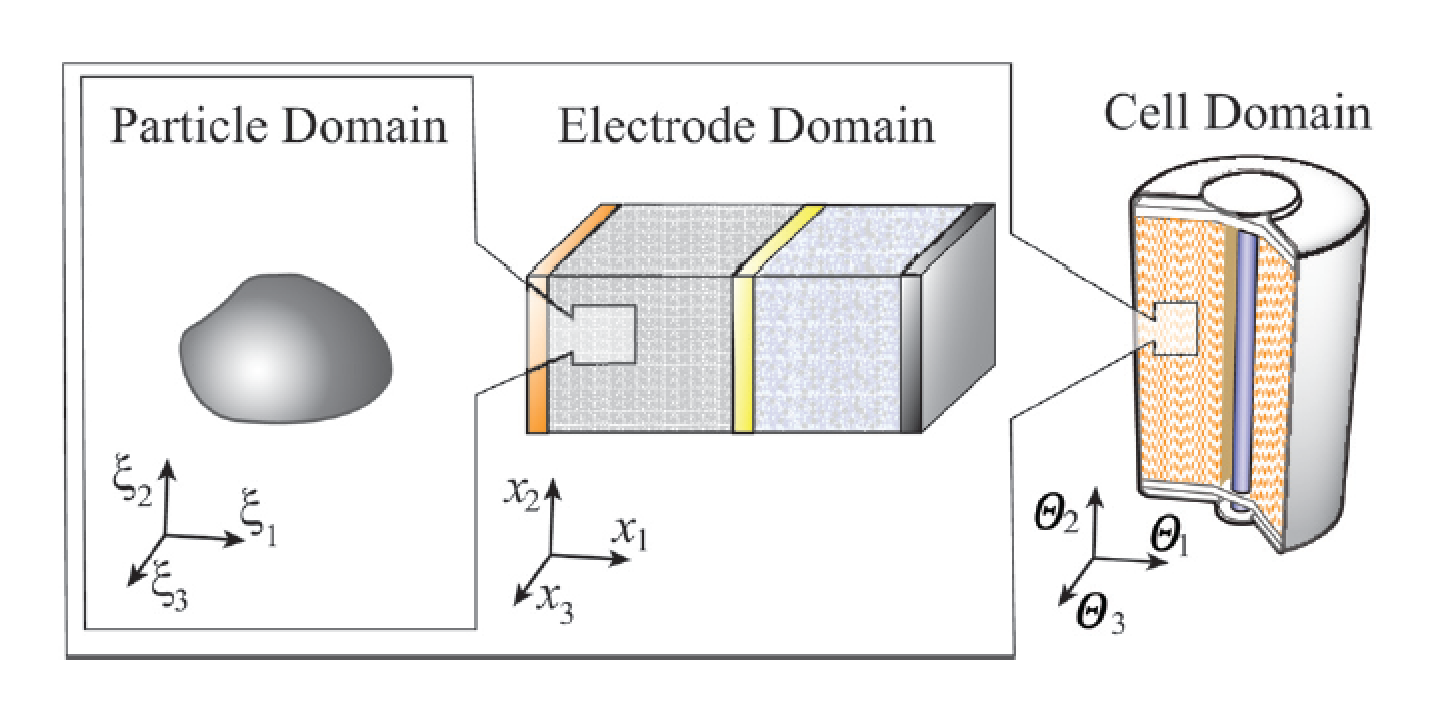
\includegraphics[width=0.5\textwidth]{msmdfig1.png}
\caption{The 3 level (i.e. 3 spatial scale) hierarchy presented in \cite{Kim-etal:2011}.}
\label{figure:batterymsmdhier}       
\end{figure}

\begin{figure}
  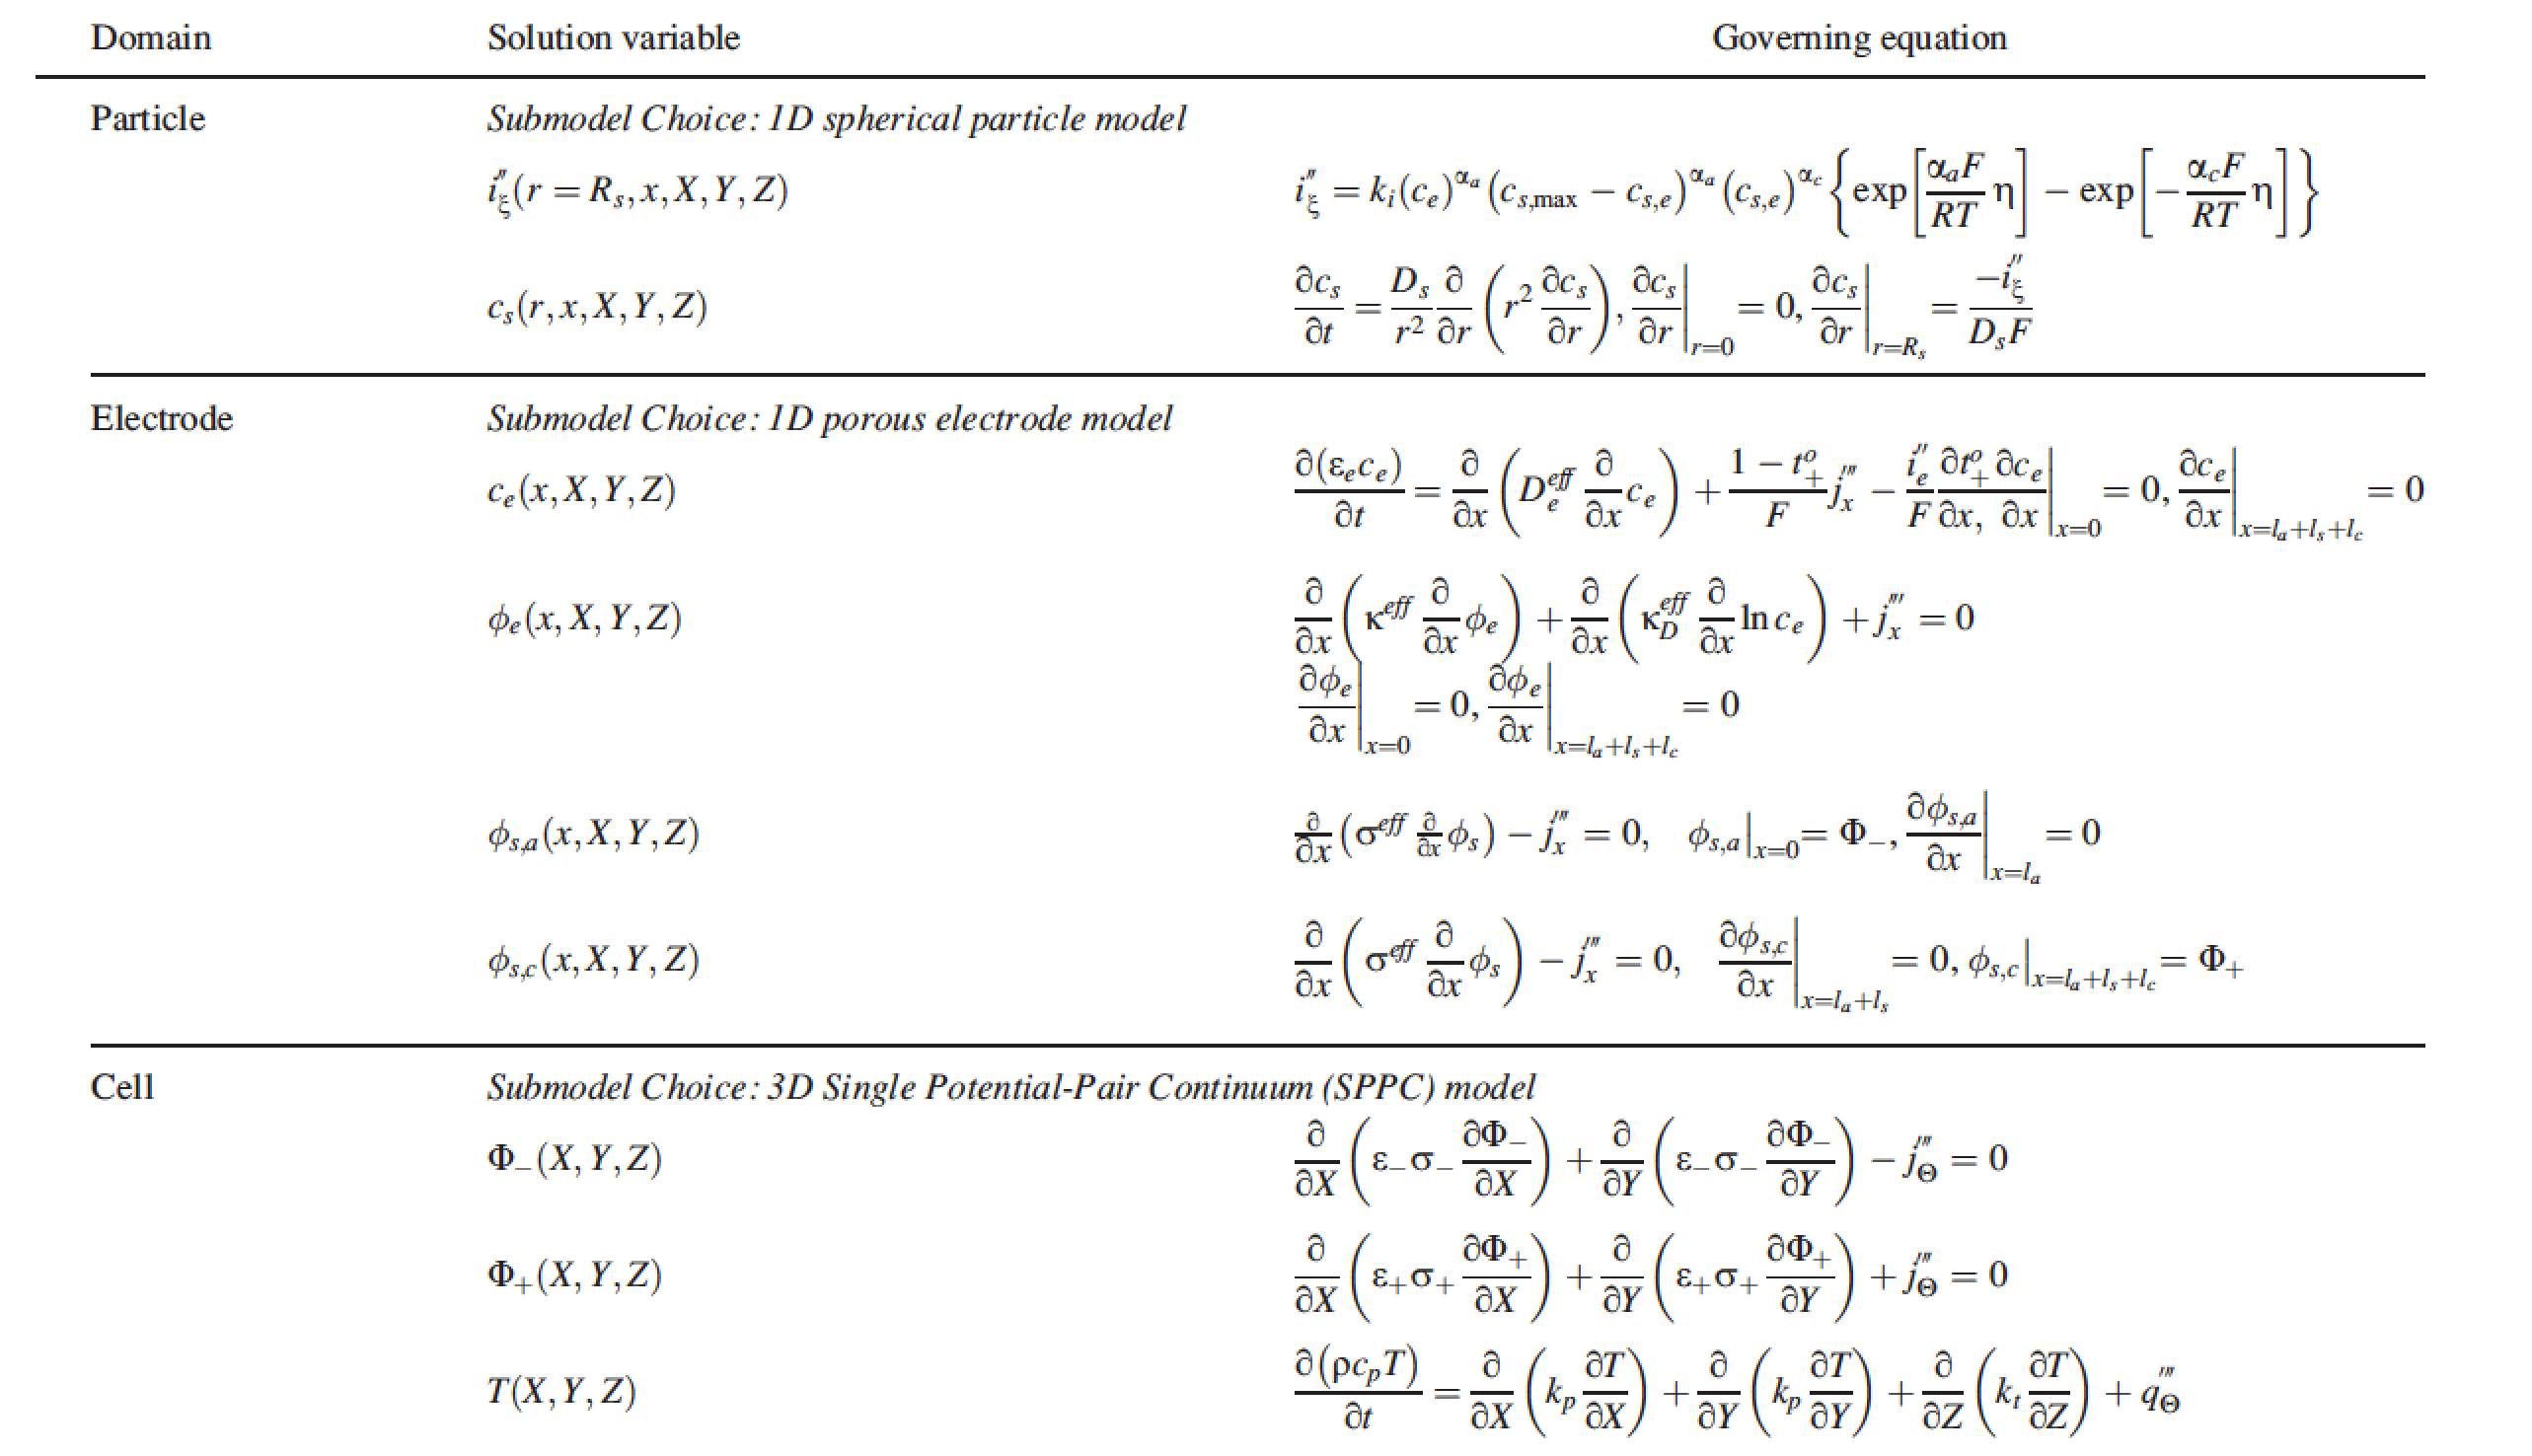
\includegraphics[width=0.9\textwidth]{msmdeqns.png}
\caption{The equations solved by the system described in \cite{Kim-etal:2011}}
\label{figure:batterymsmdeqns}       
\end{figure}

\begin{figure}
  \includegraphics[width=0.9\textwidth]{lotsofbatteryscales.png}
\caption{The scales and complexities of battery modeling from \cite{Ramadesigan:2012}.  Here ``P2D" and
``P3D" refer to ``pseudo-" two and three dimensional simulations.  What this means is that (for example,
in the 2D case), the discretization of a 1D electrode model contains 1D subgrid models at every grid point.}
\label{figure:fullhierarchy}       
\end{figure}


\subsubsection{Hierarchies in battery simulation and modeling}

The most obvious hierarchy in battery modeling is across spatial scales (battery operation involves 8-10 orders of magnitude):
As stated above, MSMD uses 3 \emph{separate} domains (cell, electrode, particle) [a 4th scale, ``pack", is in the works],
i.e. ``sub-grid" PDE models at each volume element, each of whose volume elements also contain sub-grid PDE models.
These communicate ``down" by boundary conditions and ``up" by
source terms.  

Roughly, the three levels in MSMD have three levels of experiment that correspond to them.  At the cell level, we can probe for
temperature (T), current (I), and voltage (V).  To some extent it is possible to measure their spatial dependence, but this is an expensive measurement we want to make as infrequently as possible.  At the electrode level, we can measure the effective diffusivity 
of Li transport.  At the particle level, we can measure the diffusivity of Li ions in Li-hosting particles.

But there are more subtle hierarchies.  For example,  
across levels of complexity for the same parameter:  Every measured parameter is associated with a model; nothing 
is \emph{directly} measured.  Thus all measured parameters are \emph{effective} parameters.
This is exemplified by measuring the Li- diffusion constant, $D_s$, of a Li-hosting particle. 
Most common is measurement of what is clearly the \emph{effective} diffusivity in an entire
electrode (containing thousands/millions(??) or particles), by current voltage measurements across the whole electrode.
  On another ``scale", we measure $D_s$ 
by literally constructing a single particle ``battery" and measuring its characteristics.  Even this represents an effective
diffusion of the particle(s) in this arrangement.  For example, we can further refine this by performing a 
different measurement and extract the \emph{anisotropic} diffusivity.  Even so, we must finally recognize that what is happening
in the particle is not even necessarily diffusion at all (grain boundaries, trapping, electrostatics, etc., may all be in play).
It is always a \emph{model} that allows us to back out $D_s$ from what we measure.  Given $D_s$ derived at one ``scale" (e.g., 
a single particle system), it is not clear how to translate that into the $D_s$ derived from, say, a full electrode model.
But that is a subject of our proposal.

Other examples:
\begin{itemize}
\item Sharp points enhance Li-plating: (this can be good, but is mostly bad).  This can be measured, but not in situ.  It can also be
simulated, but at increased computational expense.  This is an example of a complex measurement that adds
information, but that we would want to do selectively.
\item A hierarchy similar to that for $D_s$ exists for the electrolyte diffusivity, $D_e$.  At the highest level, a simple formula based on cell dimensions, thickness, and porosity is used to estimate $D_e$.  Next we derive $D_e$ is by recognizing that it is a function of the viscosity of the many chemicals that make up the composition of the electrolyte. 
\item  There is a hierarchy used to work from one parameter to the next.  At the electrode level, one needs to \emph{first} 
know $D_s$ in order to use an electrode model to estimate $D_e$ (the model from which $D_e$ is derived uses $D_s$).
\item  The use of frequency sweeps: more complex experiments involving current voltage measurements over a range of frequencies allows
extracting parameters from more complex (presumably more realistic) models.
\item An interesting point perhaps specific to batteries is a rather overt justification of
 the use of effective parameters: the many particles sandwiched between the electrodes constitute an
electrically parallel circuit; the parallel circuit ``spreads" the charge, i.e., the
system naturally equilibrates, resulting in an averaging associated with the existence of plausible effective parameters.
\end{itemize}

Our battery modeling colleagues reminded us that throughout, we must consider 
``observability": is the experiment sufficient to determine the parameter?

\subsection*{Issues in battery modeling}
Following \cite{Ramadesigan:2012}, here are four specific issues deemed to be especially important:
\begin{itemize}
\item Sparsity of manipulated variables.  The only variables
that can be manipulated during battery operation to make best use
of the battery is the charging current profile and operating temperature

\item Need for better fundamental models to understand SEI-layer,
structure.  The physicochemical understanding is incomplete for
much of the phenomena that occur inside a battery, such as capacity
fade, stress-strain effects, mechanical degradation, and mechanisms
for failure due to shocks, defects, and shorts.

\item Robustness and computational cost in simulation and
optimization.  Battery models result in multiple DAEs to be simulated
with unknown initial conditions while operating for multiple
cycles of charge and discharge.

\item Uncertainties in physicochemical mechanisms.  
No existing model simulates all of the mechanisms for capacity
fade or battery failure. More detailed information is required
to sufficiently specify a hypothesized mechanism for a phenomenon
before it can implemented in a simulation model.
Conventional degradation models based on extensive testing of
batteries under various operating conditions and loads have in general
attributed the degradation of battery performance to loss of the active
material and loss of lithium that can be cycled.
\end{itemize}

Table (\ref{table:batteryexpscales}) is a compilation of several important properties and the
relevant measurements at each scale.  Our methodology allows simultaneous incorporation of data and 
models on all the scales.
\begin{table}[htdp]
\caption{Multiscale battery measurements.  Our multi-scale Bayesian framework allows coupling of the
all the data and all the data available on all the scales.}
\begin{center}
\begin{tabular}{|p{1.5in}|p{1.5in}|p{1.5in}|p{1.5in}|}
\hline
property  & microscale & mesoscale & macroscale \\
\hline
\hline
diffusivities & single-crystal measurements, molecular diffusivity  \cite{Chung:2011} & in-situ/single particle measurements \cite{Cui:2012} & GITT/PITT (Routinely carried out using composite electrodes) \cite{Wen01121979}
 \\
%Multi-scale measurements hel p resolve disputes in transport mechanism

\hline
 rate constants  &
reactive TEM� (PNNL) & 
Aurbach and others & 
EIS (only ``effective reactivities" are of interest to the macro-models) \\
%Multi-scale measurements help eliminate multiple �optima�

\hline
open circuit potentials, entropy measurements, decomposition potentials  &
composition versus lattice structure (e.g., XRD Ceder, Ohzuku) &
ECQM???  &
C/50 discharge\\
%�Voltage fade�???, non-stoichiometric �phases�???, hysteresis!!!, decompn. potentials fairly well documented

\hline
Conductivities (electronic, ionic) &  
quantum transport   &
Measure properties of individual components and use mixing rules (effective medium theory) &
Measure effective conductivities \\
%Not strictly multiscale; need to think about this more

\hline
mechanical properties &
in-situ TEM \cite{Wang:2012} &
single particle and in situ electrode level \cite{Qi:2010,Verbrugge:1999} &
pressure transducers  \\
%Rational design across scales

\hline
\end{tabular}
\end{center}
\label{table:batteryexpscales}
\end{table}%



\subsection{Formulation of multi-scale implicit sampling for modeling pressure in battery systems}
\MarginPar{PETER: I envision this being \emph{after} the disussion of the formalism; i.e. not necessarily
in the same place that we discuss batteries in general}
The fluctuation of pressure with time can critically affect performance, degradation, and safety of batteries.
Referring to Table (\ref{table:batteryexpscales}) we label the scales at which to model battery processes
somewhat arbitrarily as ``micro-" (nanometers), ``meso-" (microns), and ``macro" (millimeters-).  
Referring to the above general formulation of multi-scale implicit sampling,  let the state/parameters
at these scales be denoted $x^0$, $x^1$, and $x^2$, respectively.
  The macroscale state variable $x^2$ of interest is pressure.  We can measure it via data $y^2$ which consists
of detailed signals from transducers.  
%For purposes of this discussion, we can assume the ``observation model" 
%$y^2 = h(x^2) + \textrm{ noise}$ is perfect, so $y^2 \equiv $x^2$   
  Macroscale pressure is in fact the manifestation of many effects at the mesoscale: conversion of electrolyte
to the gas phase; the sponge like nature of the porous electrode; elastic properties of the binder (the binder
is the "glue" that holds the particles in their porous structure); the porosity and toruosity of the separater.  The pressure is the sum of all these effects combined across the whole cell.  Let $x^1$ represent the state,
described at the mesoscale in terms of such quantities as layer thicknesses (substrate, epoxy layer,
current collector, active material, entire electrode), volume fractions (particles, binder, pores), 
porosity, tortuosity, particle sizes and distributions  
(see, e.g., \cite{Sethuraman2012334}) and other parameters governing the makeup and morphology of the heterogeneous
electrode.
Let $y^1$ be data
gathered regarding mesoscale phenomena such as stress, strain, swelling, and other mechanical properties.  
Our goal is to
incorporate all available data, i.e. both $y1$ (measuring electrode properties: stress, strain, etc.) and $y2$ (measuring cell properties: pressure), into the estimate of
$$
	p(x^2,x^1 | y^2,y^1) \propto p(y^2|x^2) p(x^2|x^1) p(x^1),
$$
the conditional expection of cell-level pressure and electrode-level stress and strain, given both
cell and electrode level data.
The first term on the right hand side represents our observation model of "pressure".
The second term come from a physical or statistical model of how the various mesocsale quantities 
affect pressure.  The last term is our guess at what the mesoscale parameters really will be.
From this equation we can see how both the data (first term) and physical model (second term) are being
incorporated.  

To sample from this distribution by implicit sampling, we will follow the steps outlined above, specifically:\\
form $F = -\log( p)$\\
minimize it, get $\sigma_F$, or even (from a population based algorithm) $\{\sigma^i_F\}_{i=1}^{Npop}$\\
sample from it by repeatedly\\
 -- sample $\xi$ from Gaussian\\
 -- solve $F-\sigma_F = \xi^T \xi$. \\
With these samples in hand we can calculate any desired statistics of the macroscale pressure. 
What have we accomplished?  We have demonstrated a formulation that allows physics-based models (e.g., 
how pressure arises from mesoscale phenomena) to inform our interpretation of macroscale measurements. 
Conversely, we have demonstrated how the physics-based model can ``learn" from the macroscale measurements.

Interestingly, we can also reverse the formulation.  This is perhaps more of interest, in fact, because
macroscale pressure measurements are \emph{more} reliable than meso- and micro-scale measurements.  By applying
the formalism from scale $2$ emph{to} scale $1$, we have 
$$
	p(x^1,x^2 | y^1,y^2) \propto p(y^1|x^1) p(x^1|x^2) p(x^2).
$$
In this case the physics model is used to compute $p(x^1|x^2)$.  Because of the presumed (in this case)
many-to-one relation between mesoscale parameters and macroscopice pressure, this term acts as more
or a constraint (what $x^1$ is compatible with $x^2$) than a prediction (what is $x^2$, given $x^1$).

Proceeding further down in scale, at the microscale we can incorporate data from electronic structure calculations,
for example, the effect of 
Li- "loading" on the lattice constants of the crystals in the electrode (e.g., $\textrm{CoO}$).
Here, $x^0$ represents a choice of compound (and perhaps crystal structure), and the data $y^0$ are profiles of
lattice constant values versus Li-loading.  DFT calculations are performed to accomplish the
``measurement" of $y^0$ (i.e., $p(y^0|x^0)$.).  The "scale coupling" model $p(x^1|x^0)$ comes, for example, from 
mean field theory [ref].  Thus we can assimilate the data from all three scales on estimates of pressure 
via
$$
	p(x^2,x^1,x^0 | y^2,y^1,y^0) \propto p(y^2|x^2) p(y^1|x^1) p(y^0|x^0) p(x^2|x^1) p(x^1|x^0) p(x^1) p(x^0).
$$
For a specific, known compound $x^0$, we have
$$
	p(x^2,x^1 | y^2,y^1,x^0) \propto p(y^2|x^2) p(y^1|x^1) p(x^2|x^1) p(x^1|x^0) p(x^1).
$$
\MarginPar{need to check these exact formulae.}
Now, the model represented by the term $p(x^1|x^0)$ is a function of the lattice constants $y_0$, so it involves
DFT calculation, followed by modeling of the mesoscopic parameters w.r.t. the lattice constants and
other values that come out of it.  
This is one of many example of interest.  Table (\ref{table:batteryexpscales}) summarizes several
such multi-scale data hierarchies in battery research

Having $p$ factored in this form allows implicit sampling to be applied to draw samples from this joint 
distribution.  
In this way statistics of pressure can incorporate models and measurements on all three scales.
We propose to further develop this example, to assess the validity of assumptions (1) and (2) above [IN THE 
FORMULATION SECTION], and
study the implementation of implicit sampling in this context.
This is likely a case where derivatives of models with respect to parameters is not directly possible
through adjoints.  But, the formulation involves paramters, not states, so the problems are not
high-dimensional.  We will pursue derivative free optimization (DFO) for equation (XXX) above in this case.

The use of DFO represents another research path applied to this example.  In particular,
many DFO algorithms utilize a ``population" of candidate solutions.  
(e.g., covariance matrix adaptation evolutionary strategy (CMA-ES) \cite{hansenrankmu,cmaes},
as well as of course traditional evolutionary algorithms such as genetic algorithms, etc).
There is thus an obvious connection to be explored between the set of particles being used in the overall
data assimilation problem, and the population (of particles, we may say) being used in the DFO.
Of special interest is the CMA-ES algorithm as it involves
 dynamically identifying scales on different axis and exploiting
this knowledge in optimization (i.e. converting long thin valleys of search space into bowls); this
is clearly related to ``affine sampling", discussed elsewhere in this
proposal ([WHERE?])

\bibliography{batteries2}
\bibliographystyle{plain}


\end{document}
